\chapter{Entwurf}\label{chapter:entwurf}
Dieses Kapitel beschäftigt sich mit dem Entwurf des Prototyps. Die Aufgabe des Entwurfes eines Softwaresystems ist es aus den gegebenen Anforderungen softwaretechnische Lösungen zu entwickeln \citep{balzert:softwaretechnik}. Die Grundlage bilden dabei die in Kapitel \ref{chapter:Anforderungsanalyse} definierten Anforderungen.

\section{Allgemeine Technologieentscheidungen}
Im ersten Teil des Entwurfs werden grundlegende Technologieentscheidungen betrachten, die die Grundlage für das folgende Design bieten.

\subsection{Anwendungsart}
Die Anwendung soll Lernenden eine weitere Zugriffsmöglichkeit auf Wissensinhalte in Form von Augmented Reality bieten.
Wie bereits in den Anforderungen festgelegt, soll dafür die Anwendung auf einem mobilen Endgerät laufen.\\
Dieses bietet im Bezug auf AR mehrere Vorteile. Zum einen ist es wichtig, dass das Endgerät frei im Raum bewegbar ist, damit der Anwender gut mit den AR-Objekten interagieren kann. Dieses ist durch ein mobiles Endgerät gewährleistet. Eine Alternative dazu wären sogennante Head-Mounted-Displays (siehe Kapitel \ref{sec:HMD}). Diese besitzen aber im Vergleich eine deutlich geringere Verfügbarkeit. Ein Handy oder Tablet besitzt dagegen heutzutage fast jeder Student und hat dieses auch so gut wie immer parat. Dadurch ermöglicht ein Smartphone zusätzlich einen schnellen, ortsunabhängigen Zugriff. \\
Ein weiteren Vorteil den ein mobiles Endgerät mit sich bringt ist die Kamera verfügt, welche für die meisten Trackingverfahren essentiell ist. \\

\subsubsection{Betriebssystem}
Für mobile Anwendungen gibt es vor allem zwei Plattformen, die für diese Arbeit in Frage kommen. Auf der einen Seite steht Apples IOS und auf der Anderen Android von Google. Insgesamt gibt es im Bezug auf die AR-Anwendung nicht viele Argumente, die für eine bestimmte Seite sprechen. Letztendlich wurde Android als Zielsystem gewählt, da bereits ein Endgerät, welches dieses Betriebssystem nutzt, vorliegt. Dadurch kann die entwickelte Software direkt auf diesem Gerät getestet werden. 

\subsubsection{Entwicklungsumgebung}
Basierend auf der Entscheidung das Betriebssystem Android zu nutzen, wurde die Entwicklungsumgebung (IDE) wurde Android Studio gewählt, weil dieses die offizielle Entwicklungsumgebung für Android Anwendungen darstellt und viele praktische Features bereitstellt. 

\subsection{Trackingverfahren}
Für Augmented Reality Anwendungen auf einem Smartphone kommen vor allem visuelle Tracking Verfahren, bei denen das Kamerabild als Eingabe für den Tracker genutzt wird, in Frage. Dabei gibt es jedoch nochmal die Unterscheidung zwischen Natural Feature Tracking und Markerbased Feature Tracking (vgl. Kapitel \ref{sec:Trackingverfahren}). \\ 
Für den konkreten Anwendungsfall dieser Arbeit ist das markerbasierte Verfahren am besten geeignet. Es ermöglicht, dass Speichern von Informationen über den Identifikator (ID) der einzelnen Marker. Dadurch kann man jedem individuellem Marker ein AR-Objekt zu ordnen. Diese Zuordnung ist mit Hilfe von natürlichen Bildpunkten nicht direkt möglich, da bei diesem Verfahren lediglich ein Objekt im Bild positioniert wird und anhand markanter Bildpunkte der Umgebung ausgerichtet und transformiert wird. \\
Ein weiterer Vorteil den die Marker bieten ist dass sie sich einfach in verschiedene Arten von Dokumenten einbinden lassen und dann im Anschluss lediglich mit Hilfe einer Kamera eingescannt werden müssen. 

\subsection{Tracking Bibliothek}
Mittlerweile gibt es viele Bibliotheken, die Methoden und Klassen zur Umsetzung von Augmented Reality bereitstellen und die Tracking Verfahren müssen nicht selbst erstellt werden. Jedoch unterstützen nicht alle von Ihnen auch das Markerbasierte Verfahren. Eines der vermutlichen bekanntesten Bibliotheken, die die Anforderungen erfüllen, ist ARToolKit. Es stellt umfangreiche Klassen zur Implemtierung von Augmented Reality zur Verfügung und unterstützt dabei die verschiedensten Markervarianten von simplen Hiro Markern bis hin zu Barcode Markern mit verschiedenen IDs.
Im Rahmen dieser Arbeit wurde die Version ARToolKitX genutzt. \\
Weitere mögliche Bibliotheken wären Googles ARCore, welches jedoch keine explizite Marker Unterstützung besitzt, oder OpenCV, welches viele Methoden zum Tracken bereitstellt, jedoch im Vergleich zu ARToolKit einen deutlich aufwendigeren Implementierungsprozess benötigt. ARToolKit bietet zusätzlich den Vorteil, dass es bereits an die Konzepte von Android angepasst wurde und sich somit gut in die bestehende oder neue Android Anwendungen einfügen lässt.


\section{Designentscheidungen}
Im folgenden Abschnitt werden konkrete Designentscheidungen für die Implementierung der Anwendung getroffen.

\subsection{Grundlage der Entwicklung}
ARToolKitX stellt neben dem Methoden und Klassen zur Umsetzung von Augmented Reality auch eine simple AR-Anwendung bereit, die die zuvor definierten allgemeinen Technologieentscheidungen erfüllen kann.\\
Diese Anwendung kann als Grundlage für die folgende Implementierung genutzt werden und im Rahmen dieser Arbeit so erweitert werden kann, dass sie die in Kapitel \ref{chapter:anforderungsanalyse} entwickelten Anforderungen erfüllt.\\ 
Die Anwendung von ARToolKit \glqq ARSquareTrackingExample\grqq{} trackt einen einzelnen Hiro-Marker und projiziert einen bunten Würfel auf den Marker. \\
Damit die gestellten Anforderungen erfüllt werden können, müssen in der Implementierung die folgenden, grundlegenden Punkte umgesetzt werden:
\begin{enumerate}
\item Marker: Die genutzen Hiro-Marker der Anwendung können keine ID speicheren. Also müssen andere Marker verwendet werden. Des weiteren muss die Anwendung die Marker selbst generieren können, damit der Nutzer eigene Modelle Tracken kann.

\item Modelle: Die Anwendung verfügt lediglich über ein einzelnes hardgecoded Modell, welches angezeigt werden kann. Dieses muss durch das Laden eigener, variabler Modelle ersetzt werden.

\item Texturen:  Auch die Textur die in Form fest definierter Farben im Text verankert ist muss, durch das Laden und anwenden der Texturdatei ersetzt werden.

\item Datenspeicherung: Basierend auf den beiden vorherigen Punkten muss die Anwendung ein Konzept zur Speicherung der hochgeladenen Modelle imnplementieren, damit diese dem Nutzer auch nach einem Neustart der Anwendung zu Verfügung stehen.

\item User Interface: Die Anwendung von ARToolKitX besitzt noch kein User Interface, sie zeigt lediglich die Kamera und rendert das Modell in dieses Bild. Damit die finale Anwendung jedoch alle Funktionen erfüllen kann muss ein User Interface zur Navigation zwischen den einzelnen Komponenten eingeführt werden.
\end{enumerate}
Im folgenden werden die aufgeführten Punkte einmal genauer betrachtet und konkrete Designentscheidungen getroffen.

\subsection{Marker}
Die Hauptanforderung an die Marker ist, dass sie über eine ID differenziert werden können. ARToolKitX stellt hier die sogenannten Barcode-Marker bereit, die aus einem schwarzen Rand und einem Pattern, das eine codierte ID beinhaltet, bestehen. Diese Marker sind speziell auf das Tracking von ARToolKitX zugeschnitten und sollen auch in der Implementierung genutzt werden. \\
Bei der Verwendung dieser Marker müssen zwei Entscheidungen getroffen werden.\\
Zum einen muss über die Größe des Patterns entschieden werden. Hierbei unterstützt ARToolKitX Matrizen der der Größe 3x3 bis 6x6. Die Größe der Matrix beeinflusst dabei die Anzahl der Marker, die generiert werden sollen. Dabei sind kleinere Matrizen vermutlich jedoch weniger fehleranfällig. \\
Der zweite Eigenschaft, die variieren kann ist die Codierung der Marker. Dazu nutzt ARToolKitX je nach Matrixgröße verschiedene Codierungsmethoden, die den Sinn verfolgen die Fehlertoleranz, bei Auslesen des Patterns, zu erhöhen. Dieses geschieht indem sich die einzelnen Marker durch die Codierung optisch deutlicher unterscheiden. Zwar ist die Fehlertoleranter des Trackings umso höher je größer die Unterschiede sind, allerdings sinkt dadurch auch die Anzahl der verschieden Marker.\\
Da die Fehleranfälligkeit zu Beginn noch nicht eingeschätzt werden kann, werden zunächst einmal die simplen 5x5 BarcodeMarker ohne Codierung genutzt. Allerdings sollte bei der Implementierung auf eine leichte Austauschbarkeit der Marker geachtet werden, um auf mögliche Probleme reagieren zu können.

\subsection{Modelle}
Da es dem Nutzer mit der Anwendung möglich sein soll eigene Modelle hochzuladen, muss die Software die entsprechenden Dateien einlesen und verarbeiten können. Für diese Modelldateien stehen dem Nutzer verschiedene Datei-Formate zur Verfügung. Der zu entwickelnde Prototyp soll zunächst lediglich das OBJ-Format unterstützen, dieses könnte dann in der Zukunft recht einfach erweitert werden. \\
Diese Entscheidung beruht darauf, dass dieses Format von den meisten Grafikprogrammen unterstützt wird. So ist es auch mit dem kostenlosen Tool Blender, welches zum Erstellen der Testmodelle genutzt wurde, möglich die Objekte im OBJ-Format zu exportieren und somit auch andere Formate in das OBJ-Format zu konvertieren. \\
Eine weitere Anforderung an das Modell ist, dass die sogenannten Faces, welche die einzelnen Flächen (Polygons), trianguliert werden. Dieses ist in den meisten Grafikprogrammen ohne Probleme vor dem Export möglich. Auch hier könnte in späteren Versionen des Prototyps über eine erweiterte Unterstützung nachgedacht werden.

\subsection{Texturen}
Neben der OBJ-Datei bestehen die Modelle die in diesem Format exportiert werden aus einer Materialdatei und einer Textur in Form einer Bilddatei.\\
Beide stellen eine Variante dar um einem Modell eine Textur zuzuweisen.\\
Für den Prototyp wurde die Entscheidung getroffen, die MTL-Datei, welche Materialinformationen des Objektes speichert nicht zu betrachten, sondern dem Nutzer die Möglichkeit zu bieten, die Textur des Modells über eine Bilddatei zu definieren.\\
Diese Entscheidung beruht zum einen auf der Tatsache, dass die viele der Modelle die Online zur Verfügung stehen primär auf diese Variante zurückgreifen und zum Anderen das Erstellen eines eigenen Modells mit einer Texturdatei für einen Nutzer, ohne Vorkenntnisse im Bereich der Modellierung, einfacher ist.


\subsection{Datenspeicherung}
Die Anwendung muss die Modelle, die vom Anwender hochgeladen werden auf geeignete Weise abspeichern.\\
Da dieses zunächst nur auf lokaler Ebene passieren soll, kann für diesen Zweck auf den internen Speicher zurückgegriffen werden. Dieser bezeichnet den Speicher der einer Anwendung und dessen Inhalt bei Deinstallation der Anwendung gelöscht wird. \\
Zusätzlich muss noch eine Referenzierung über die MarkerID auf den zugehörigen Speicherort der kopierten Dateien im internen Speicher erfolgen, damit zum einen alle Modelle beim Start der Anwendung geladen werden können und zusätzlich jedem Modell ein Marker zugeordnet ist.
 
\subsection{User Interface}
Damit der Nutzer auf alle Funktionen des Prototyps zugreifen kann, soll dieser simples User Interface besitzen, welches dem Nutzer grundlegende Interaktionsmöglichkeiten bietet. Ein erstes Mockup dieses Interfaces wird in Abbildung \ref{fig:ui-mockup} dargestellt.
\begin{figure}[h!]
\centering
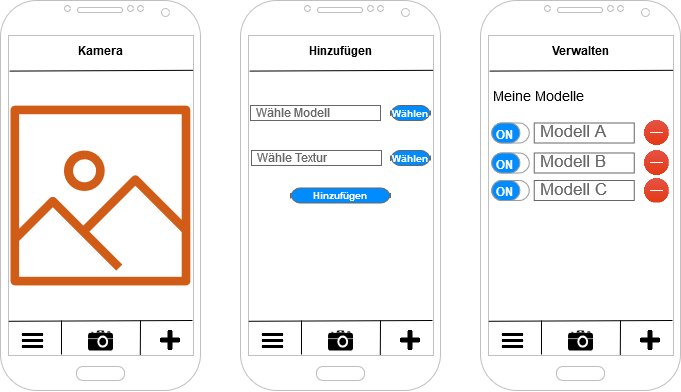
\includegraphics[width=0.8\textwidth]{Abbildungen/ui-mockup.png}
\caption[UI Mockup]{Das Mockup des User Interfaces. (Quelle: Eigene Darstellung)}
\label{fig:ui-mockup}
\end{figure}
Es zeigt die drei Ansichten (Fragments) der Anwendung, welche von der Navigation überlagert werden. \\
Die Navigation besteht aus zwei Teilen am oberen Bildschirmrand ist der Titel des aktuellen Fragments zusehen und am unteren Rand befindet sich die eigentliche Navigation. Diese besteht aus drei repräsentativen Icons, welche jeweils ein Fragment repräsentieren. Über einen Druck auf den entsprechenden Knopf erscheint die zugehörige Ansicht.\\
Das Hauptfragment stellt die Kamera dar. Hier wird das Kamerabild analysiert und mittels Augmented Reality, um die entsprechenden Objekte erweitert. Zusätzlich ist noch ein Fragment zum Hinzufügen von Modellen und eins zum Verwalten der Fragments vorgesehen.\\
Letzteres bietet dem Nutzer die Möglichkeit bestehende Modell wieder zu entfernen.
